\documentclass[border=10pt]{standalone}
\usepackage{amsmath} % for \dfrac
\usepackage{physics}
\usepackage{pgfplots}
\usetikzlibrary{decorations.pathmorphing} 
\usetikzlibrary{angles,quotes} % for pic (angle labels)
\usetikzlibrary{arrows,arrows.meta}
\usetikzlibrary{calc}
\usetikzlibrary{decorations.markings}
\pgfplotsset{compat=1.18}


\colorlet{Bcol}{violet!90}
\colorlet{BFcol}{red!70!black}
\colorlet{veccol}{green!45!black}
\colorlet{Icol}{blue!70!black}
\colorlet{Ampcol}{green!60!black!70}

\begin{document}
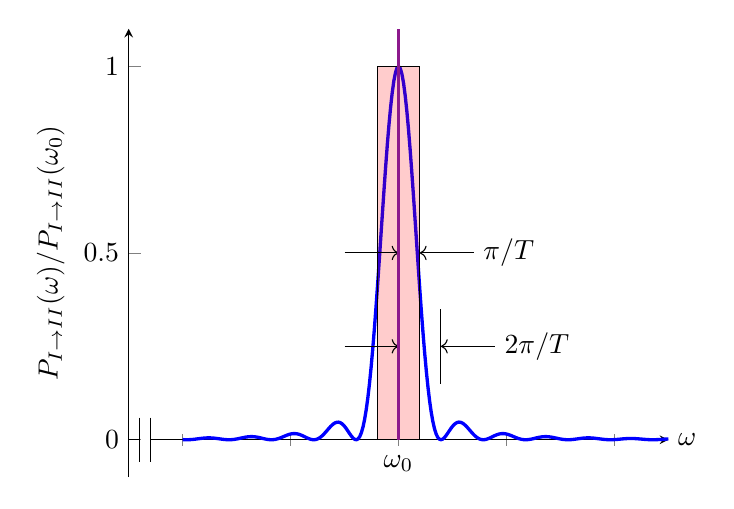
\begin{tikzpicture}
    \def\wz{5}
    \def\Tw{4}
    \def\ppi{3.141592}
    \begin{axis}[
        axis y line = center, axis x line = middle,
        xmin = 0, xmax = 10, ymin=-0.1, ymax = 1.1, clip = false,
        ytick align=inside,
        xtick={1, 3, 5, 7, 9},
        xticklabels={, , $\omega_0$, , },
        axis x discontinuity=parallel, % 핵심 옵션: 평행 빗금
        ytick={0,0.5,1},
        hide obscured y ticks=false,
        xlabel style={anchor=west, at={(ticklabel* cs:1.0)}},
        ylabel style={rotate=90, anchor=near ticklabel, at={(ticklabel cs:0.5)}},
        xlabel=$\omega$,
        ylabel=$P_{I \to II}(\omega)/P_{I\to II}(\omega_0)$,
    ]
    \addplot[blue, very thick, domain=1:10, samples=300]
        {x == \wz ? 1 : (sin(deg(\Tw*(x-\wz)))/(\Tw*(x-\wz)))^2};
    \filldraw[fill=red, fill opacity=0.2, ] (axis cs:\wz-\ppi/\Tw/2, 0) -- (axis cs:\wz-\ppi/\Tw/2, 1) -- (axis cs:\wz+ \ppi/\Tw/2, 1) -- (axis cs:\wz + \ppi/\Tw/2, 0) -- cycle; 
    \draw[->] (\wz-1, 0.5) -- (\wz, 0.5);
    \draw[->] (\wz+ \ppi/\Tw/2 +1, 0.5) node [right] {$\pi/T$}-- (\wz+ \ppi/\Tw/2, 0.5);

    \draw[] (\wz+ \ppi/\Tw , 0.15) -- (\wz+ \ppi/\Tw , 0.35);
    \draw[->] (\wz-1, 0.25) -- (\wz, 0.25);
    \draw[->] (\wz+ \ppi/\Tw +1, 0.25) node [right] {$2\pi/T$}-- (\wz+ \ppi/\Tw, 0.25);

    \draw[Bcol, thick] (\wz, 0) -- (\wz, 1.1);
    \end{axis}
\end{tikzpicture}
\end{document}